\documentclass{beamer}
\usetheme{Berkeley}

\title{Disc 4a}
\author{Andy}
\institute{UC Berkeley}
\date{\today}

\begin{document}

\begin{frame}
  \titlepage
\end{frame}

\begin{frame}
  \frametitle{Minilecture: Computability}

    \begin{definition}
      Computability asks can a problem be solved via algorithm (computers)?
    \end{definition}


    \begin{enumerate}[<+->]
      \item Can we have a program that tells us if another program halts?
      \item Is there a perfect antivirus?
      \item Perfect compression algorithm?
    \end{enumerate}

\end{frame}

\begin{frame}
  \frametitle{Minilecture: Computability}

    What is a computer?
  
    \begin{figure}
      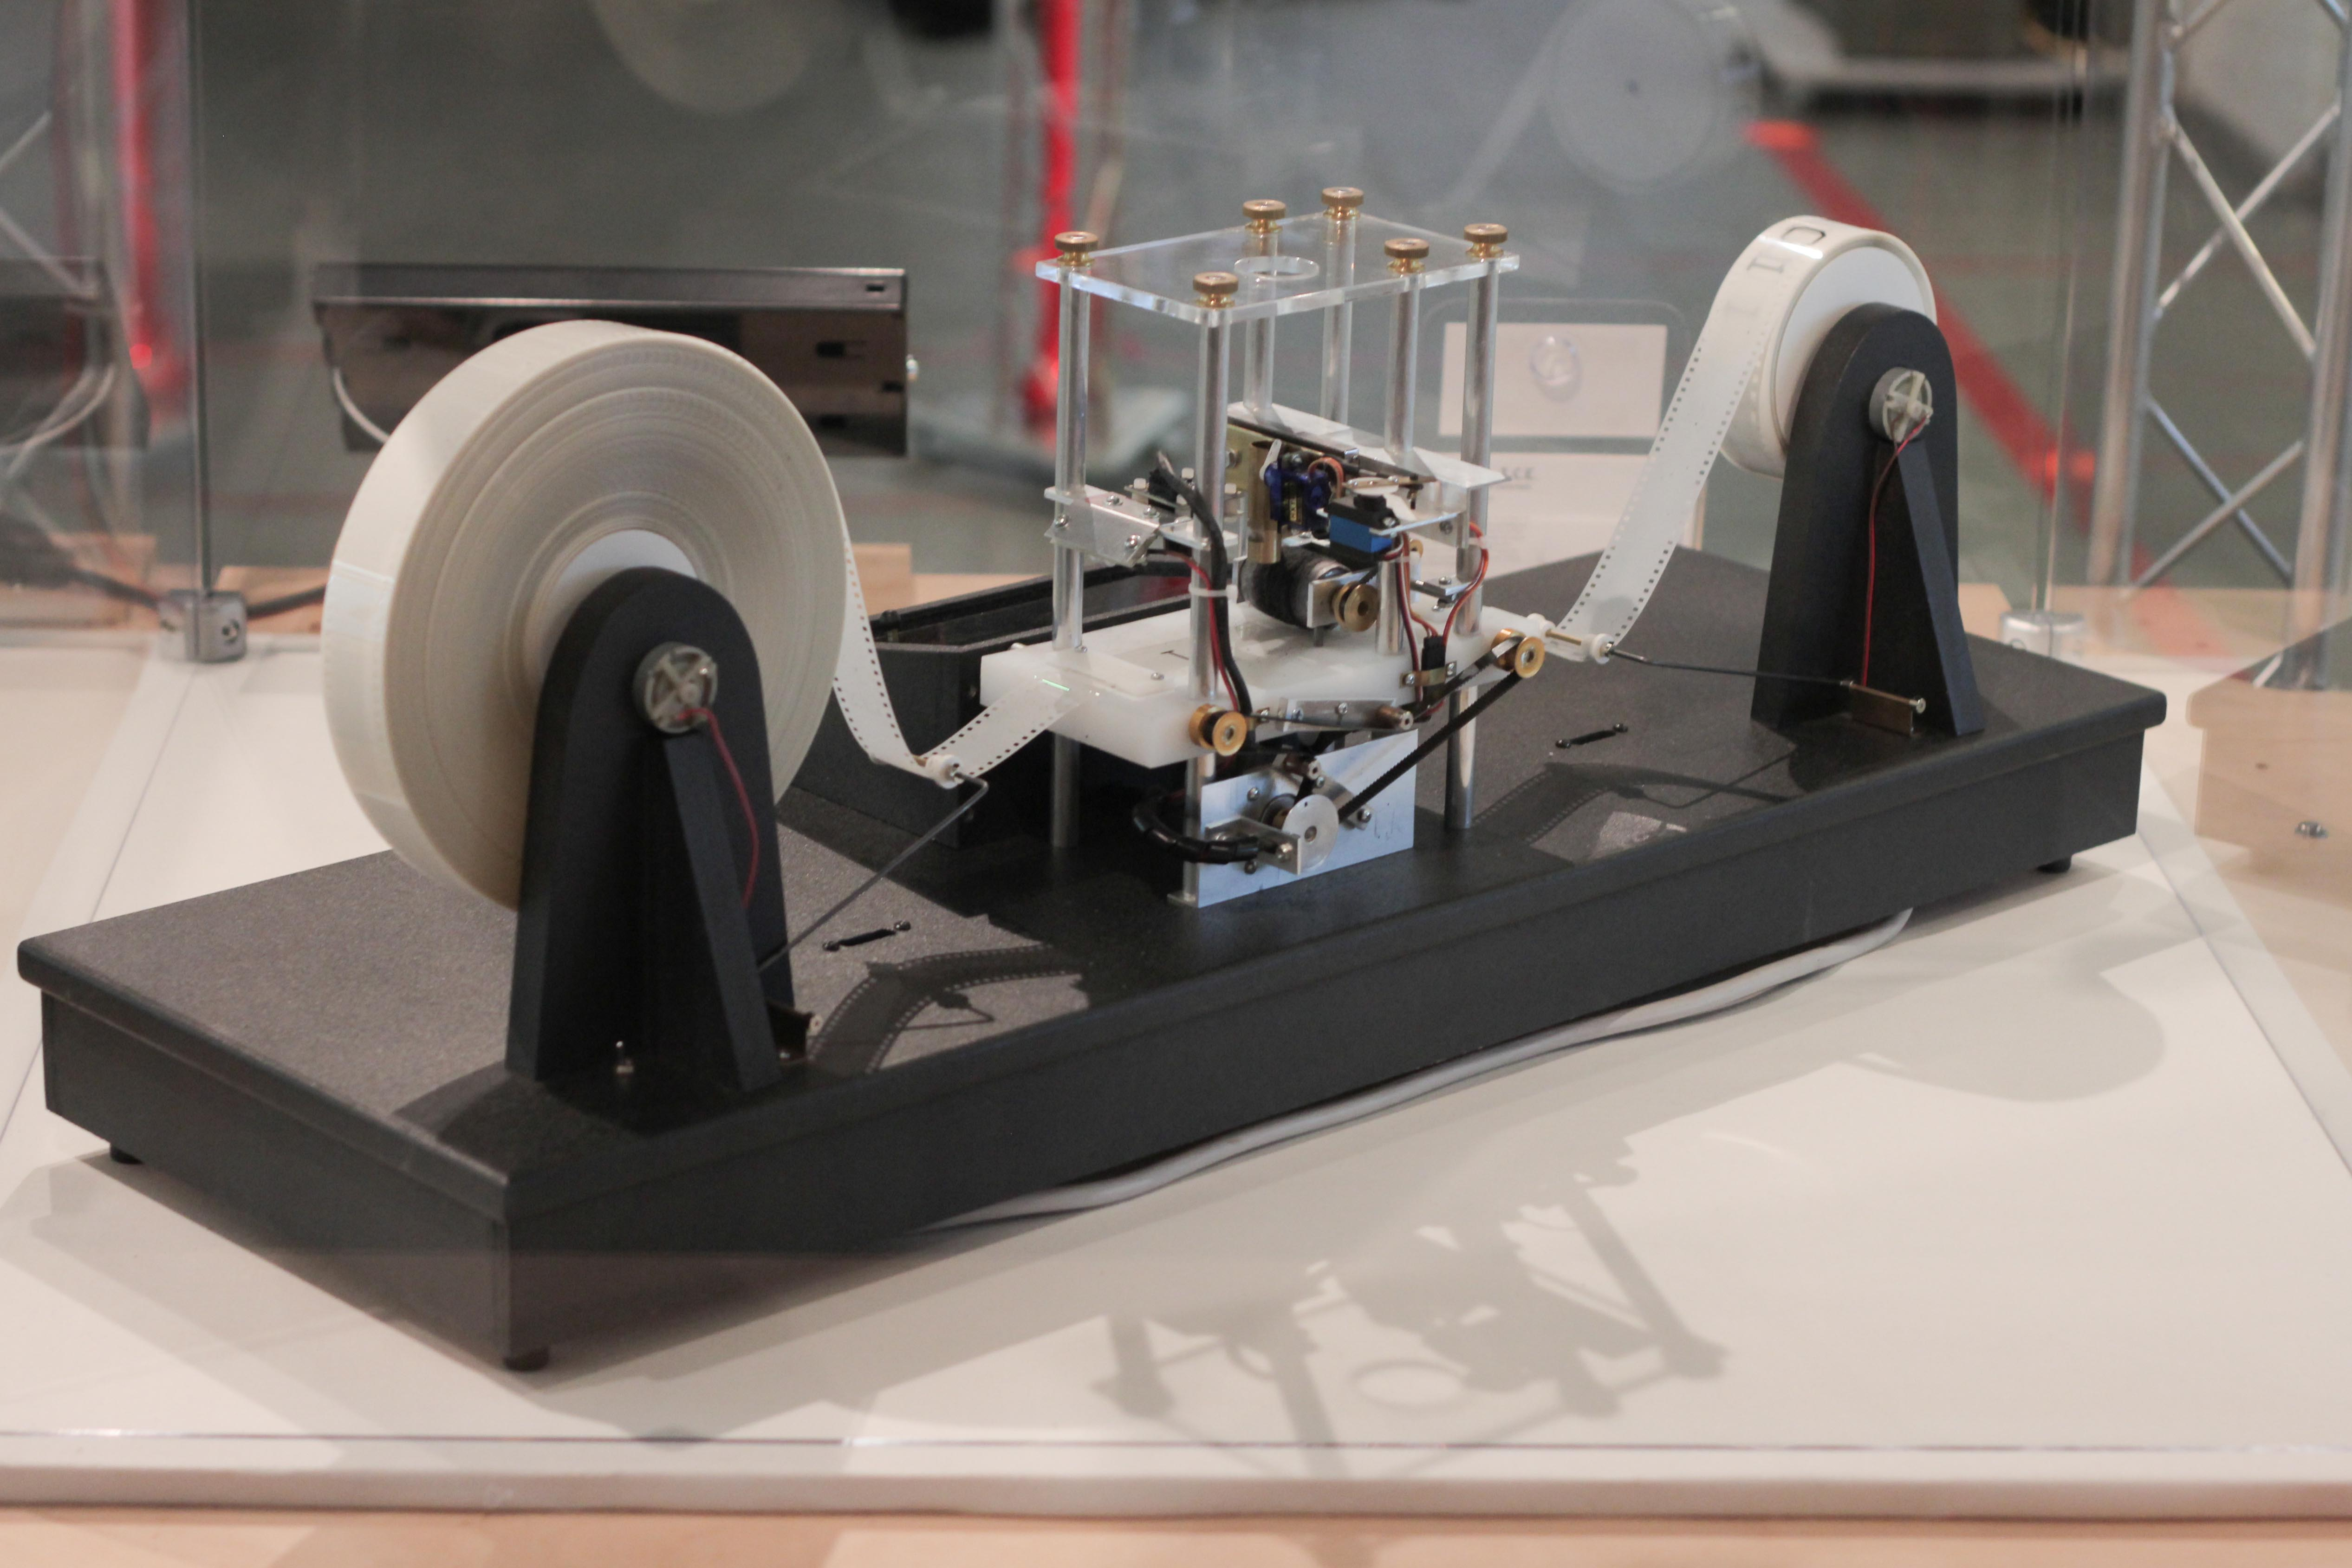
\includegraphics[scale=0.125]{turing.jpg}
      \caption{Turing Machine}
    \end{figure}

    \begin{enumerate}[<+->]
      \item Has memory. Ideally infinite memory.
      \item Has a head that can read memory
      \item Head can write 1 or 0 to memory
      \item Head decides what to do based on memory.
     \end{enumerate}
     

\end{frame}


\begin{frame}
  
  
  \frametitle{Assumptions}

  \begin{enumerate}
    \item Computers have infinite compute
    \item Computers have infinite memory
    \item But computation still takes time
  \end{enumerate}


\end{frame}

\begin{frame}
  
  
  \frametitle{Halting Problem}

  \begin{enumerate}[<+->]
    \item \alert{"This statement is false"}
    \item Can we have a program that determines if another program halts?
    \item Assume we have a program, TestHalt, that takes in P and x, and will tell you if P(x) halts
  \end{enumerate}


\end{frame}


\begin{frame}[fragile]
  \frametitle{Including Code}
  \begin{semiverbatim}
    def Turing(P):
      if TestHalt(P, P):
        loopforever();
      else:
        halt();
  \end{semiverbatim}
  
  \begin{enumerate}[<+->]
    \item We run Turing(Turing)
    \item If Turing(Turing) halts, then Turing(Turing) loops...
    \item If Turing(Turing) loops, then Turing(Turing) halts...
    \item Paradox
    \item We cannot have a paradox. If you can build a Testhalt -> paradox
    \item Anything that allows you to build a TestHalt program is impossible
  \end{enumerate}
\end{frame}

\end{document}
